% !TeX spellcheck = en_US
\addscenariosection{1}{Cooperative Scenario}{Sentinels}{\images/sentinel.png}

\begin{multicols}{2}

\textbf{Author:} silence70011

\textbf{Source:} \href{https://discord.com/channels/740870068178649108/1233112440322002964/1233112440322002964}{Archon Studio Discord}

\textit{There is a world beyond ours, filled with beasts and monsters, barely contained by a formation of four sacred Obelisks.
  But the power of these stones is waning, and a breach is imminent.
  When it happens, only you and your ally will stand between the hordes and the total devastation of these lands.
}

\subsection*{\MakeUppercase{Scenario Length}}

This Scenario is played over 12 Rounds.

\subsection*{\MakeUppercase{Player Setup}}

\textbf{Player Count:} 2

\textbf{Starting Resources:} 10 \svg{gold}, 2 \svg{building_materials}, 1 \svg{valuables}

\textbf{Starting Income:} 10 \svg{gold}, 2 \svg{building_materials}, 1 \svg{valuables}

\textbf{Starting Units:}
\begin{itemize}
  \item A Pack of \svgunit{bronze} Units with the \textit{lowest} Recruitment cost
  \item A Few \svgunit{bronze} Units with the \textit{highest} Recruitment cost
\end{itemize}

\textbf{Town Buildings:} \svgunit{bronze} Dwelling, Citadel

\textbf{Map Tile Pool:} Each player takes 1 random Near (IV--V) Map Tile and 1 random Far (II--III) Map Tile. These Tiles should not contain any Obelisks.

\textbf{Additional Bonus:} Search (2) the Artifact Deck

\subsection*{\MakeUppercase{Map Setup}}

Take the following Map Tiles and arrange them as shown in the Scenario map layout:

\textbf{2 × Starting (I) Map Tile}
\begin{itemize}
  \item Starting Tiles of your chosen Factions
  \item Ignore their yellow borders
\end{itemize}

\textbf{4 × Far (II--III) Map Tile}

\textbf{4 × Near (IV--V) Map Tile}
\begin{itemize}
  \item All Near Map Tiles must have Obelisks
\end{itemize}

\subsection*{\MakeUppercase{Victory Conditions}}

Defeat all invading armies.

\subsection*{\MakeUppercase{Defeat Conditions}}

An undefeated enemy army remains at the end of Round 12.

One of your Towns is captured, or a Main Hero is defeated in a battle (retreat doesn't count).

\subsection*{\MakeUppercase{Timed Events}}

\textbf{\nth{6} Round:}
\begin{itemize}
  \item Remove all Black Cubes from every Windmill, Water Wheel, and Mystical Garden on the map.
  \item Spawn an enemy army following the rules outlined below.
\end{itemize}

\textbf{\nth{7} and \nth{8} Rounds:}
\begin{itemize}
  \item Spawn an enemy army following the rules outlined below.
\end{itemize}

\textbf{\nth{9} Round:}
\begin{itemize}
  \item Repeat the Timed Events of Round 6.
\end{itemize}

\textbf{\nth{10} Round:}
\begin{itemize}
  \item Repeat the Timed Events of Rounds \mbox{7 and 8.}
\end{itemize}
\vspace{-0.5em}

\subsection*{\MakeUppercase{Additional Rules}}

\begin{itemize}
  \item Players can trade resources when one of the active player's Heroes Visits a trading post or stands on a Field adjacent to an allied Hero.
  \item The Hero who defeats an enemy army gains 2 \svg{experience}.
    The victorious player rolls two Treasure Dice and resolves one of them.
  \item Additionally, no player can:
  \begin{itemize}
      \item Attack other Heroes.
      \item Capture a Mine or Settlement that is already Flagged.
  \end{itemize}
\end{itemize}

\subsection*{\MakeUppercase{Enemy Spawning\\and Movement}}

\begin{itemize}
  \item Enemy armies spawn on a random Obelisk Field (use Hero miniatures from Factions not in play).
  \item Determine which Obelisk Field by rolling 2 Attack Dice. Apply the results as follows (D1/D2), reroll any 0:
  \begin{itemize}
    \item $+1$/$+1$ = North
    \item $+1$/$-1$ = East
    \item $-1$/$+1$ = West
    \item $-1$/$-1$ = South
  \end{itemize}
  \item For a more balanced distribution, in Rounds 7 and 9, only roll the second Attack Die (D2). For D1, take the opposite result from what was rolled in the previous Round.
  Rounds 8 and 10 are entirely random.
  \item If the Tile where an enemy is to spawn hasn't been discovered yet, flip it over and orient it as preferred.
  \item If there is a Hero on the Field where the enemy spawns, a fight starts immediately.
  \item Enemy armies move at the end of every Turn, starting with the Turn they spawned.
  \item Enemy armies have 3 MPs per Round.
  \item Enemy armies move as described in the rulebook (p.\,33), but instead of capturing, they destroy everything in their path.
    Place Black Cubes on any Field they pass through, treating those Fields as empty from that point on.
  \item If an enemy's movement could go in different directions, the players decide which way they go.
\end{itemize}

\subsection*{\MakeUppercase{Combat with\\Enemy Armies}}

\begin{itemize}
  \item Fighting enemy armies over more than one Combat Round does not cost Movement Points.
  \item During a battle with an enemy army, a Hero can retreat whenever a friendly Unit is about to Activate.
    A retreating Main Hero loses all remaining MPs and is returned to an allied Town or Settlement of their choice, keeping all remaining Units.
  \item Retreating Secondary Heroes are removed from the game, but their remaining Units are kept.
  \item Killed enemy Units do not respawn.
\end{itemize}

\subsection*{\MakeUppercase{Boss Army}}

\begin{itemize}
  \item In Round 10, a Boss Army spawns. It is different from previous armies because it is Reinforced from a fixed pool of Neutral Units (Reinforcement pool = number in brackets in the table below).
  \item At the beginning of the \nth{2} Combat Round and every following Round, 2 Units Reinforce the remaining army from the shuffled reinforcement pool (up to a maximum of 5 Units) to continue the fight until either the player retreats or every Neutral Unit from the Reinforcement pool is killed. \textit{If the number of enemy Units at the beginning of a Round is 1 or lower, draw up to a total of 4 Units (i.e., there are always 4 or 5 enemy Units on the Board after Reinforcing, if available).}
  \item Place the Reinforcing Units on the enemy base line, starting from the left with the lowest Initiative (\svg{unit_ranged} Units first). If necessary, continue on the next line in the same order.
  \item When a player retreats, the enemy army draws up to the ``minimum'' of 4 Units and takes these as starting Units to the next fight.
\end{itemize}

\columnbreak

\vspace*{\fill}

\end{multicols}

\begin{tikzpicture}[overlay]
  \centering
  \node at (14, 2) {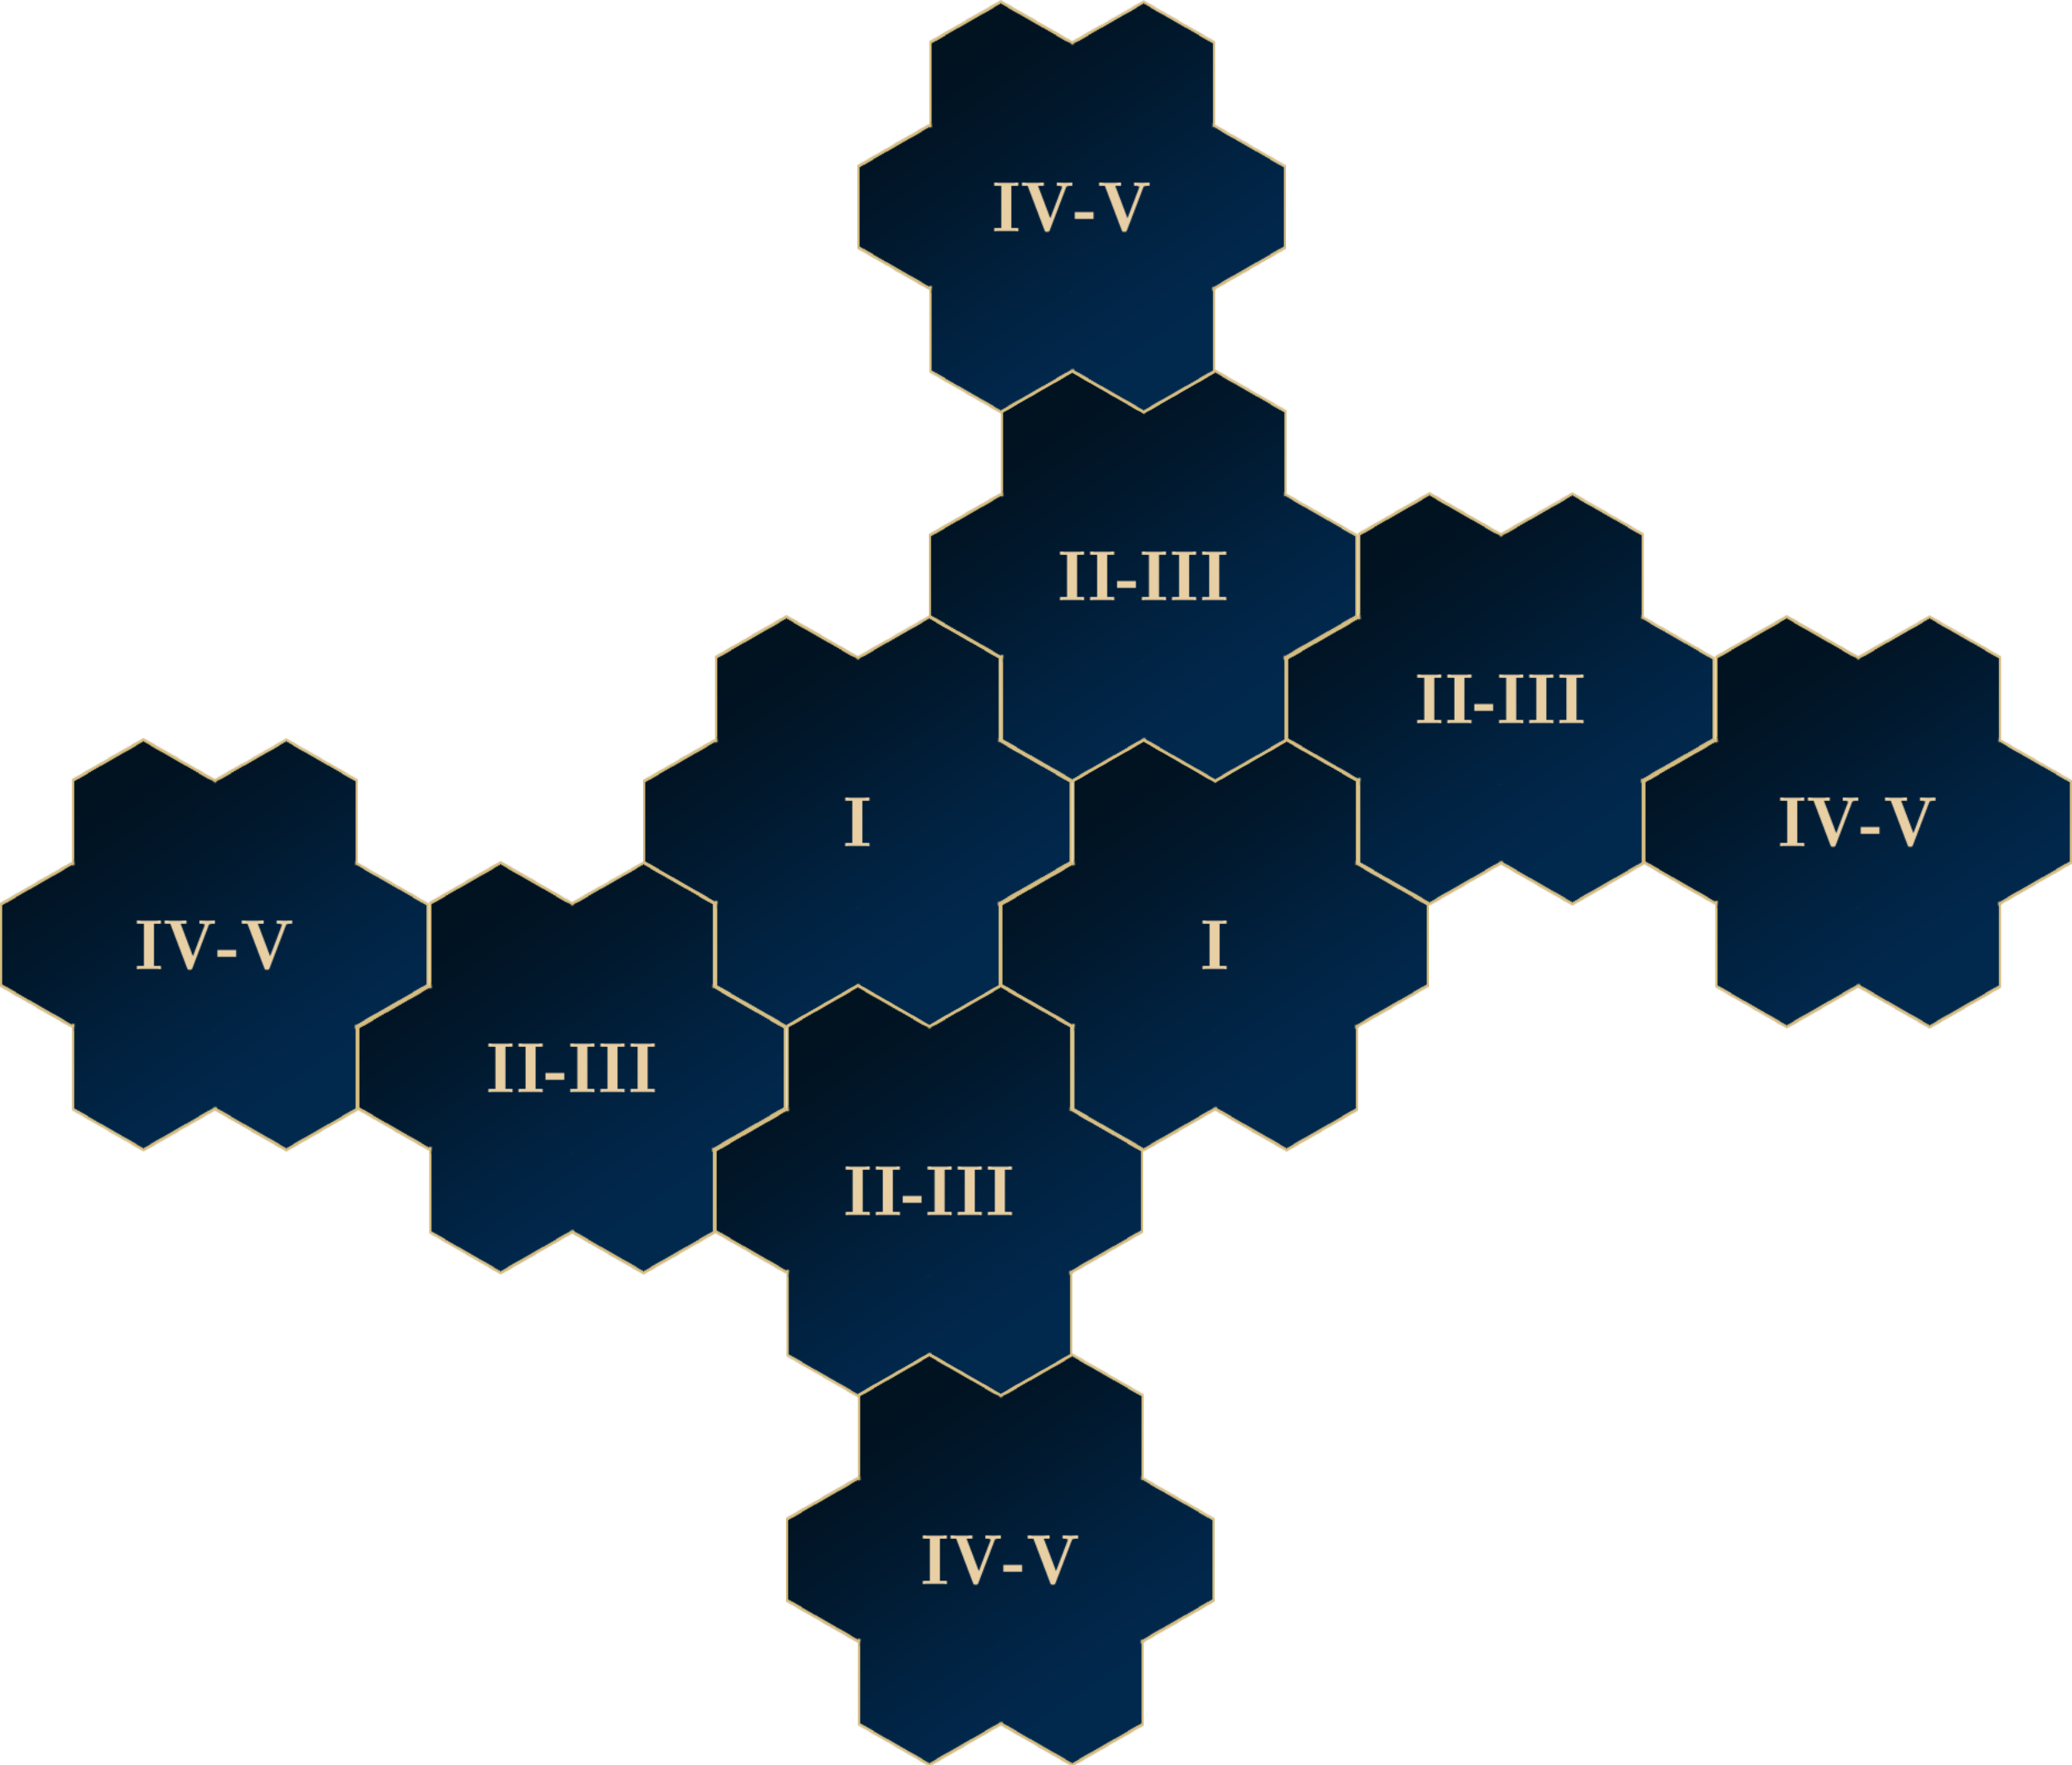
\includegraphics[width=0.4\paperwidth]{\maps/sentinels.png}};
\end{tikzpicture}

\vspace*{\fill}

\hommtable[]{20}{
  \centering
  \medskip
  \textbf{Strength of Enemy Armies}\\
  \bigskip

  \newcommand{\bronze}[0]{\svgunit[12]{bronze}}
  \newcommand{\silver}[0]{\svgunit[12]{silver}}
  \newcommand{\golden}[0]{\svgunit[12]{golden}}
  \newcommand{\azure}[0]{\svgunit[12]{azure}}

  \begin{tabularx}{\linewidth}{p{0.15\linewidth}XXXX} & \darkcell{Rounds 6 + 7} & \darkcell{Rounds 8 + 9} & \darkcell{Round 10}\\
  \darkcell[1.4]{Easy}
    & \lightcell[1.4]{\bronze \silver \silver \silver \golden}
    & \lightcell[1.4]{\silver \silver \silver \golden \golden}
    & \lightcell[1.4]{\silver \silver \golden \azure \footref{azure} \linebreak
      (2\bronze, 4\silver, 3\golden, 1\azure)}\\
  \darkcell[1.4]{Normal}
    & \lightcell[1.4]{\silver \silver \silver \golden \golden}
    & \lightcell[1.4]{\silver \silver \silver \golden \azure}
    & \lightcell[1.4]{\golden \golden \golden \azure \footref{azure} \linebreak
      (2\silver, 7\golden, 1\azure)}\\
  \darkcell[1.4]{Hard}
    & \lightcell[1.4]{\silver \silver \golden \golden \golden}
    & \lightcell[1.4]{\silver \silver \golden \golden \azure}
    & \lightcell[1.4]{\golden \golden \azure \azure \footref{azure} \linebreak
      (2\silver, 6\golden, 2\azure)}\\
  \darkcell[1.4]{Impossible}
    & \lightcell[1.4]{\silver \golden \golden \golden \golden}
    & \lightcell[1.4]{\golden \golden \golden \golden \azure}
    & \lightcell[1.4]{\golden \azure \azure \azure \footref{azure} \linebreak
      (7\golden, 3\azure)}\\
  \end{tabularx}
}

\vspace*{\fill}

\footnotetext[1]{Always 1 Unit of Azure Dragons (starting Units of Boss Army). The rest is random\label{azure}.}
